\chapter{概述}\label{ch:overview}

\section{简介}\label{sec:1-introduction}

在现代嵌入式系统（Embedded
System）中，随着对计算要求的增长，多核系统的普遍性在快速增加，同时异构计算的趋势也越发显著。同时，架构显著相异的微控制器系统的功能复杂度和市场占有率快速提升，而对资源管理的要求也在增长。但是，对于多核系统，在计算能力增长的同时，其实时性往往因为资源访问竞争而受到影响，因此有必要编写无锁化、少共享态的全并行内核；对于微控制器（Microcontroller
Unit，MCU）系统，其内存管理方法各异，传统的抽象方法往往不能满足需求，而无法使用和中大型计算机相同的系统级编程范式，因此有必要新编写一个系统来统一内存管理接口。

同时，在现代高性能系统中，轻量级虚拟化功能的重要性逐渐增加。在大型服务器中虚拟化可以使资源管理更加灵活，更可以实现诸如虚拟机热迁移等应用，方便硬件维护；在高性能嵌入式系统中，虚拟化（Virtualization）可以允许微控制器或数字信号处理器（Digital
Signal
Processor，DSP）安全地运行第三方二进制代码，或者运行多个高级语言虚拟机，而不会造成安全和资源控制问题。在两种场景中，都要求虚拟机响应实时、具备高效率，并且可伸缩可扩展。

RME（RTOS-Mutate-Eukaron）实时操作系统（Real-Time Operating
System，RTOS）是一种极度可伸缩（Scalable）、可扩展（Expandable）的全抢占式微内核实时操作系统。它提供了第三代微内核所提供的所有特性：灵活的用户态调度器，完善的底层存储管理，高效的通信机制以及针对特定硬件的特殊优化能力。RME 操作系统可以在仅具 64kB 只读存储器（Read-Only Memory，ROM）和16kB随机读写存储器 （Random-Access
Memory，RAM)的微控制器上运行，同时也可以在具备上百个CPU插槽和几百TB内存的高性能服务器上运行，并且拥有同样优越的运行效率。

\subsection{设计目标}\label{subsec:1-design-goals}

作为第三代微内核，RME 的设计目标主要包括以下四点：灵活性，安全性，可靠性和实时性。

灵活性（Flexibility）意味着系统可以适应于多种应用场景，并在运行于多种架构情况下充分发挥各种架构的潜力，同时又使用尽量多的通用部分。为此，RME 在设计时考虑到了从微控制器到超级计算机在内的一系列可能平台，并遵循了严格的编码兼容性规范来适应各种可能的编译环境。

安全性（Security）意味着系统中各类资源的受控的保密性（Confidentiality），完整性（Integrity）和可用性（Availability）。为了达到上述三点要求，RME 将权能（Capability）作为系统的根基。这意味着，在系统中，一切都是由权能（Capability）控制和管理的；如果要对内核对象进行操作，那么必须通过系统调用，传入相应的权能进行操作。在用户态，不同的内核对象管理器管理不同类别的权能，因此它们的耦合性很低，相互之间的隔离程度也因此较高。

可靠性（Reliability）意味着系统中很少或没有功能性错误，并在此类错误发生时能够进行子系统的微重启（Micro-reboot）。作为微内核，RME 先天比宏内核来得可靠；为尽量减少错误的发生，RME 的架构无关部分代码都经过全分支覆盖的白盒测试。

实时性（Real-time
Responsiveness）意味着系统中所有的执行路径都是有确定时限约束的，并且这些时限都是较短而不至造成问题的。RME 在设计时考虑到了所有执行路径的可预测性，即使在多核环境下也能维持自身的硬实时性。

\subsection{软件版权与许可证}\label{subsec:1-copyright-and-license}

综合考虑到微控制器应用、深度嵌入式应用和传统应用对开源系统的不同要求，RME 内核本身所采用的许可证为 Unlicensed，但是对一些特殊情况\footnote{比如安防器材和医疗器材等}使用特殊的规定。
这些特殊规定是就事论事的，对于每一种可能情况的具体条款都会有不同。

\subsection{易混术语表}\label{subsec:1-terms-and-definitions}

在本书中，容易混淆的基本术语规定如下：

\subsubsection{操作系统}\label{subsubsec:1-operating-system}

指运行在设备上的执行最底层处理器、内存等硬件资源管理的基本软件。

\subsubsection{进程}\label{subsubsec:1-process}

进程指拥有一定资源的最小的独立保护空间。这些资源可以是某些内核对象、某段内存、某些设备等。通常而言，这个保护空间会对应于某个正处于执行状态的程序的实例。

\subsubsection{线程}\label{subsubsec:1-thread}

线程指操作系统中拥有一个独立执行栈和一个独立指令流的可被调度的实体。一个进程内部可以拥有多个线程，它们共享一个进程地址空间。

\subsubsection{协程}\label{subsubsec:1-coroutine}

协程指操作系统中仅拥有一个独立指令流而无独立栈的可被调度的实体。一个线程可以拥有多个协程，这些协程共享一个线程栈。

\subsubsection{静态分配}\label{subsubsec:1-static-allocation}

指在系统编译时就决定好资源分配方式的分配方式。

\subsubsection{半静态分配}\label{subsubsec:1-semi-static-allocation}

指在系统启动过程中决定好资源分配方式，并且在之后的运行中不再更改的分配方式。

\subsubsection{动态分配}\label{subsubsec:1-dynamic-allocation}

指在系统运行过程中，可以更改资源分配的分配方式。

\subsubsection{软实时}\label{subsubsec:1-soft-real-time}

指绝大多数情况下操作应该在时限之内完成，但也允许小部分操作偶尔在时限之外完成的实时性保证。

\subsubsection{硬实时}\label{subsubsec:1-hard-real-time}

指所有操作都必须在时限之内完成的实时性保证。

\subsubsection{常数实时}\label{subsubsec:1-constant-real-time}

指所有操作对用户输入和系统配置都是O(1)的，而且执行都能在某个有实际意义的常数时限之内完成的实时性保证。这是所有实时保证中最强的一种。

\subsubsection{对某值常数实时}\label{subsubsec:1-value-constant-real-time}

指所有操作和响应在某个能于系统配置决定的值不变的时候都是O(1)的，而且执行都能在某个有实际意义的常数时限之内完成的实时性保证。

\subsection{主要参考系统}\label{subsec:1-major-reference-systems}

权能表、信号端点和同步迁移调用参考了 Composite（@GWU）。

页表的部分实现参考了 Composite（@GWU）。

页表的动态页功能参考了 uCLinux（@Emcraft）。

内核内存权能的理念参考了 Fiasco.OC（@TU Dresden）。

权能的操作标志和线程的最大优先级实现参考了 seL4（@Data61/CSIRO）。

内核中的轻量调度队列实现参考了 RMProkaron（@EDI）。

系统调用接口的实现参考了 Linux（@The Linux Foundation/Linus Torvalds）。

隔离内核的实现参考了 Barrelfish（@Microsoft/ETH Zurich）。

其他各章的参考文献和参考资料在该章列出。

\section{前言}\label{sec:1-foreword}

操作系统是一种运行在设备上的执行最底层处理器、内存等硬件资源管理的基本软件。对于实时操作系统而言，系统的每个操作都必须是正确的和及时的，其执行时间必须是可预测的。总的而言，有两类实时操作系统：第一类是软实时系统，第二类是硬实时系统。对于软实时系统，只要在大多数时间之内，程序的响应在时限之内即可；对于硬实时系统，系统的响应在任何时候都必须在时限之内。实际上，很少有实时应用或操作系统完全是软实时的或者完全是硬实时的；他们往往是软实时部分和硬实时部分的有机结合。例如，LCD显示屏及人机界面部分往往是软实时的，而电机控制部分往往是硬实时的。

通常而言，绝大多数的实时系统都是嵌入式系统。嵌入式系统是指在软硬件上都高度定制化的专用系统，其对系统的性能、功耗、体积以及运行环境都有非常严苛的要求。此类系统包括了工业自动化控制器、飞行控制器、火箭控制器等的高度定制化系统和工控机等相对通用的系统。

传统上，由于硬件功能的限制，实时系统一般都比较简单，使用简易的操作系统或者不使用操作系统是可以应对的。目前，随着新一代微控制器和微处理器的上市，应用软件的复杂性大大增加了，这使得使用新一代的实时操作系统成为必然。

新一代的实时操作系统在可靠性、可移植性和灵活性等方面比现有的实时系统都要更加强大，尤其是对于多核处理器的利用和对于并行化的设计和考虑。考虑到这些设计要求，微内核是一个必然的选择。微内核实现了最小化的一套原语，可以用来将传统操作系统放在内核态的绝大多数功能放置到用户态的服务器中去。如果其中有驱动或者服务器发生了故障，我们往往能将故障限制在小范围内而不至于使其扩展到整个操作系统。因此用户态的各个服务器可以分别重启，也可以进行冗余备份，大大提高了系统的安全性和可靠性。

此外，微内核总体而言使多核并行相关的代码编写变得更加容易了，因为内核简单，需要加入的同步机制的数目更少了。这使得我们能够大量使用读-改-写（Read-Copy-Update，RCU）技术，让编写一个无锁内核成为可能。而且，由于微内核的权能都被放入表内，对齐到一个缓存行，因此我们总是能够避免缓存一致性导致的假共享（False-sharing）问题，从而大幅提高内核在多处理器或者多不对称内存访问节点架构（Non-Uniform
Memory Access，NUMA）下的性能。

我们在此回顾一下操作系统的种类。在本手册中，我们把常见的操作系统分成五类，分别称为全定制系统、超轻量系统、基本实时系统、复杂应用系统和复杂应用实时系统。下面我们将分别介绍这些操作系统的概念。

\subsection{全定制系统}\label{subsec:1-fully-customized-systems}

此类系统是针对某种应用全定制的操作系统。他们不具备一般操作系统意义上的系统服务和软件抽象层，也不具备内核空间和用户空间的区别，应用程序直接运行在裸机上。通常而言，单内核（Unikernel）都属于此类系统。绝大多数微控制器前后台裸机处理系统也属于此类系统。

典型的此类操作系统包括 Rump（单内核）和 Mirage OS（单内核）。

\subsection{超轻量系统}\label{subsec:1-ultra-lightweight-systems}

超轻量系统是能够被称为操作系统的最小系统。通常而言，它一般运行在8位机甚至4位机上面，不需要系统定时器，没有内核态和用户态的区别，并且无需移植即可在多种架构上运行。它通常仅仅由一小段负责任务切换的代码甚至是几个宏组成，不需要定制的链接器脚本即可编译运行。

它一般由一个 while() 主循环组成，然后在该循环中逐个调用任务函数。任务函数为简单的状态机，每次进入都选择一个状态运行。各个任务之间使用同一个栈。任务代码会和内核编译在一起。任务表现为互相不可抢占的合作性协程，并且不需要是可重入的。

其优先级系统是使用硬件中断的优先级配置来完成的，而在硬件中断函数中将会直接处理所有的内容，而非将它们推迟到任务中处理。中断对操作系统是完全透明的，操作系统并不需要知道中断是否已经到来。

典型的此类操作系统包括 EDI 的 RMS（超轻量协程库）和 FAU 的 Sloth（增强的轻量协程库）。

\subsection{基本实时系统}\label{subsec:1-basic-real-time-systems}

基本实时系统是初步展现了实时系统的基本特性的最小系统。它一般运行在高档8/16位机以及低档32位机上面，需要一个系统定时器。它没有用户态和内核态的区别，但是可以将内存管理单元（Memory
Management Unit，MMU）或内存保护单元（Memory Protection
Unit，MPU）配置为保护某段内存。它需要简单的架构相关汇编代码来进行上下文堆栈切换。若要使得其在多种架构上可运行，修改这段汇编代码是必须的。移植往往还涉及系统定时器，堆栈切换，中断管理和协处理器管理。此类系统可以使用定制的链接器脚本也可以不使用，通常而言在涉及到内存保护的时候必须使用定制的链接器脚本。

在此类系统中任务表现为线程。任务函数有可能是可重入的。每个任务会使用单独的执行栈。任务代码和内核代码可以编译在一起也可以不编译在一起。任务调用系统函数往往使用直接的普通函数调用，没有经由软中断进行系统调用的概念。

此类系统具备优先级的概念，并且一般实现了不同优先级之间的抢占和相同优先级之间的时间片轮转调度。此类系统具备初级的内存管理方案，并且这种内存管理方案一般基于SLAB和伙伴系统。

中断对操作系统可以是完全透明的，此时操作系统并不需要知道中断是否已经到来；如果需要在中断中进行上下文切换，那么就必须将堆栈切换汇编插入该中断函数中，此时需要用汇编代码编写中断的进入和退出。

典型的此类操作系统包括 RMP、RT-Thread、FreeRTOS、uC/OS、Salvo 和 ChibiOS。

\subsection{复杂应用系统}\label{subsec:1-complex-application-systems}

复杂应用系统是展现了操作系统的大多数特性的系统，但是它的实时性指标一般并不出众。它一般运行在32位机和64位机上面，需要一个系统定时器。它有严格的内核态和用户态的区别，而且要求运行的硬件上必须有MMU或者MPU。它需要一个相当复杂的定制的链接器脚本，而且需要大量移植才可以在新架构上运行。移植主要涉及到系统定时器，上下文/保护域切换，中断管理和协处理器管理等等。

在此类系统上，任务表现为进程，并且一个任务可以包含多个线程。由于使用了虚拟内存，任务函数是否是可重入的没有影响。内核代码和应用程序是分开编译的。系统调用通过软中断或者专门的系统调用指令\footnote{如 x86-64 的 SYSCALL、SYSRET 等}进行。

此类系统具备优先级的概念，但是实时性能则一般没有保证。

此类系统一般都有二级内存管理。在底层是对于页的管理，在上层则是由系统运行时库提供的堆栈管理。

中断对此类系统不是透明的。操作系统要求在中断的进入和退出时维护上下文寄存器，协处理器和MMU/MPU。

典型的此类操作系统包括 Windows、Linux、Minix、FreeBSD、MacOS X 和 Amiga。

\subsection{复杂实时应用系统}\label{subsec:1-complex-real-time-application-systems}

复杂实时应用系统是所有操作系统中最强大的一类。这类系统的主要特点，就是在复杂应用系统上，增加了对于实时性的保证，其内核执行的时间是完全可预测的。

典型的此类操作系统包括 RME、Composite、Fiasco.OC 等各种 L4、RTLinux 和 VxWorks。RME 就是作为此类系统设计的。因此，其设计需要考虑到的问题最多，设计难度也是最大的。

在\ref{subsec:1-basic-real-time-systems}
和\ref{subsec:1-complex-application-systems}
所述的内核的设计中，一直有两条路线，分别是宏内核（Monolithic
Kernel）和微内核（Microkernel）。前者的代表是 Linux，它把所有的系统服务都编译链接到内核空间。这样做的好处是所有的模块间调用都是简单的函数调用，没有跨保护域的开销，因此速度较快；而且内核本身能够提供较多的功能。后者的代表是各种 L4，它把所有的功能都尽力放置到用户空间，并且内核本身仅负责消息转发和调度等基本功能。在后来的微内核发展中，甚至连调度器和内核内存管理也被进一步放置在了用户空间。这样做的好处是操作系统的功能模块之间尽量隔离，具备较好的可维护性、安全性和可靠性，并且暴露给黑客的攻击面也较小，内核本身更可以经过形式化验证（Formal
Verification）来保证其正确性\hyperref[cite:1-4]{{[}4{]}}。这两种路线的典型系统架构图如下所示：

\begin{figure}[htbp]
    \centering
    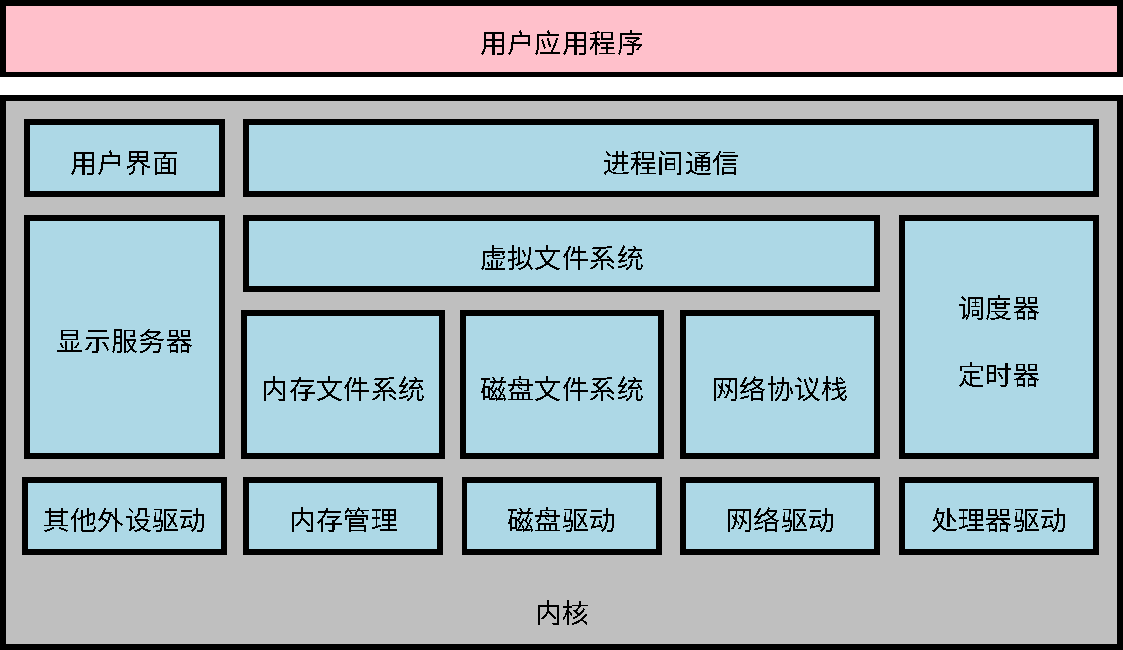
\includegraphics[width=0.72\textwidth]{Figure/image2.pdf}
    \caption{宏内核架构图}
    \label{fig:1-1-monolithic-kernel-architecture}
\end{figure}

\begin{figure}[htbp]
    \centering
    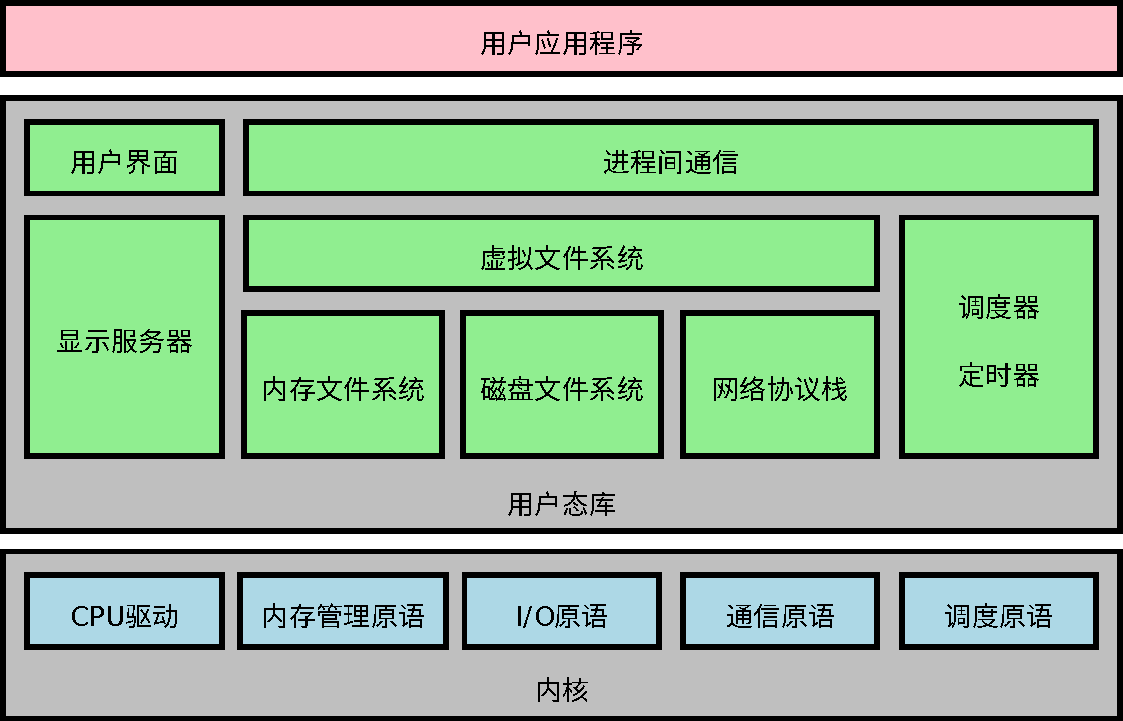
\includegraphics[width=0.72\textwidth]{Figure/image3.pdf}
    \caption{微内核架构图}
    \label{fig:1-2-microkernel-architecture}
\end{figure}

RME 采取的是微内核设计。一方面宏内核无需频繁跨保护域的优势在现代架构上已经很不明显\footnote{如最新 x86-64 的 SYSCALL 和 SYSRET 系统调用专用指令对仅消耗 60 周期，相当于一次三级缓存不命中}，另一方面微内核由于代码和数据的局部性极佳且内部结构简单而在缓存性能和并发性能上取得了决定性的优势，使得宏内核丧失了其唯一的优点------速度。新近开发的以 seL4\hyperref[cite:1-4]{{[}4{]}}为代表的一批微内核操作系统在进程间通信上可以好出 Linux 几十倍，其最坏响应时间视配置而定则要好出甚至更多。在应用程序性能上，基于微内核的网络功能虚拟化（Network
Function
Virtualization，NFV）应用也取得了普遍高出 Linux 一个数量级的性能，彻底否决了宏内核一定具有高性能的论断。

就 RME 本身而言，在某些单核架构\footnote{尤其是以 Cortex-M 为代表的一批微控制器}上的平均进程间通信性能是 Linux 的 40 倍；即便加上用户态库造成的开销，比 Linux 也要快出 25 倍。

\section{实时操作系统及其组件的性能指标}\label{sec:1-rtos-performance-metrics}

当前市场上有几百种不同种类的RTOS存在，而爱好者和个人开发的内核更是数不胜数。这些系统的性能往往是良莠不齐的。我们需要一些指标来衡量这些RTOS的性能。下面所列的指标都只能在处理器架构相同，编译器、编译选项相同的情况下进行直接比较。如果采用了不同的架构、编译器或编译选项，得到的数据没有直接意义，只具有参考性而不具有可比性。一个推荐的方法是使用工业实际标准的 ARM 或 MIPS 系列处理器配合 GCC-O2 选项进行评估。此外，也可以使用 Chronos 模拟器配合 GCC-O2 来进行评估。在评估时还要注意，系统的负载水平可能会对这些值有影响，因此只有在系统的负载水平一致的情况下，这些值才能够被比较。

\subsection{内核大小}\label{subsec:1-kernel-size}

内核的尺寸是衡量RTOS的一个重要指标。由于RTOS通常被部署在内存极度受限的设备中，因此内核的小体积是非常关键的。内核的尺寸主要从两个方面衡量，一是只读段大小，二是数据段大小。只读段包括了内核的代码段和只读数据段，数据段包括了内核的可读写数据段大小。在基于Flash的微控制器系统中，只读段会消耗Flash，而数据段则会消耗SRAM。\hyperref[cite:1-1]{{[}1{]}}

由于RTOS是高度可配置的，其内核大小往往不是固定的，而是和所选用的配置紧密相关的。因此，衡量此项性能，应该查看衡量最小内核配置、常见内核配置和最大内核配置下的内核大小。\hyperref[cite:1-1]{{[}1{]}}

内核大小数据的获得非常简单，只要用编译器编译该内核，然后使用专门的二进制查看器\footnote{如Objdump}查看目标文件各段的大小即可。

\subsection{执行时间、最坏执行时间及其抖动}\label{subsec:1-execution-time-and-jitter}

执行时间指RTOS系统调用的用时大小。最坏执行时间指执行时间在最不利条件下能达到的最大长度。RTOS的最坏执行时间通常会在如下情况下达到：执行耗时最长的系统调用，并在此过程中产生了大量的缓存未命中和快表未命中。RTOS在执行系统调用时一般都会关中断；最坏执行时间通常是系统关中断最长的时间，因此对系统的实时性的影响是非常巨大的。

最坏执行时间可以分成两类：第一类是内核系统调用的最坏执行时间，另一类是进程间通信和线程间同步的最坏执行时间。

要获得第一类最坏执行时间，可以在调用某个系统调用之前，计时器记下此时的时间戳T\textsubscript{s}，然后在系统调用结束之后，再调用计时器记下此时的时间戳T\textsubscript{e}。然后，连续调用两次计时器，记下两个时间戳T\textsubscript{ts}和T\textsubscript{te}，得到调用计时器的额外代价为T\textsubscript{te}-T\textsubscript{ts}。此时，执行时间就是T\textsubscript{e}-T\textsubscript{s}-(T\textsubscript{te}-T\textsubscript{ts})。最坏执行时间，就是所有的系统调用测试之中，执行时间最大的那一个。

要获得第二类最坏执行时间，可以在通信机制的发送端调用一次计时器，记下此时的时间戳T\textsubscript{s}，在通信机制的接收端调用一次计时器，记下此时的时间戳T\textsubscript{e}。对于调用计时器的代价测量是类似第一类最坏执行时间的。最终得到的T\textsubscript{e}-T\textsubscript{s}-(T\textsubscript{te}-T\textsubscript{ts})就是执行时间。最坏执行时间，就是所有的通信测试之中，执行时间最大的那一个。

执行时间的抖动也是非常重要的。在多次测量同一个系统的执行、通信时间时，我们往往会得到一个分布。这个分布的平均值是平均执行时间，其标准差\footnote{有时我们也使用极差}被称为执行时间抖动。

对于一个RTOS，我们通常认为执行时间、最坏执行时间和抖动都是越小越好。执行时间又可以详细分成以下几类：\hyperref[cite:1-1]{{[}1{]}}

\subsubsection{进程内线程切换时间}\label{subsubsec:1-intra-process-thread-switch}

进程内线程切换时间指在同一个进程内从一个线程切换到另外一个线程所消耗的时间。我们用下图的方法进行测量。在测量时，除了使用T\textsubscript{e}-T\textsubscript{s}的方法，也可以使用两次T\textsubscript{s}之间的差值除以2。线程切换包括两种情况，一种情况是同优先级线程之间互相切换，另外一种是由低优先级线程唤醒高优先级线程。\hyperref[cite:1-2]{{[}2{]}}

在第一种情况下，我们假设图中的两个线程是相同优先级的，而且在测量开始时，我们正执行的是刚刚由线程B切换过来的线程A。

\begin{xltabular}{\textwidth}{@{}>{\hsize=1.0000\hsize\raggedright\arraybackslash}X>{\hsize=1.0000\hsize\raggedright\arraybackslash}X@{}}
\caption{进程内线程切换的第一种情况}\label{tab:1-1-intra-process-thread-switch-case-1}\\
\toprule
进程1：线程A & 进程1：线程B\tabularnewline
\endfirsthead
\toprule
进程1：线程A & 进程1：线程B\tabularnewline
\midrule
\endhead
\bottomrule
\endlastfoot
永久循环

\{

\textgreater\textgreater{} 计时T\textsubscript{s}；

切换到线程B；

\}\strut
 & 永久循环

\{

计时T\textsubscript{e}；

\textgreater\textgreater{} 切换到线程A；

\}\strut
\tabularnewline
\end{xltabular}

在第二种情况下，我们假设图中的线程B优先级较高，而且在测量开始时，我们正执行的是刚刚由线程B切换过来的线程A。

\begin{xltabular}{\textwidth}{@{}>{\hsize=1.0045\hsize\raggedright\arraybackslash}X>{\hsize=0.9955\hsize\raggedright\arraybackslash}X@{}}
\caption{进程内线程切换的第二种情况}\label{tab:1-2-intra-process-thread-switch-case-2}\\
\toprule
进程1：线程A & 进程1：线程B\tabularnewline
\endfirsthead
\toprule
进程1：线程A & 进程1：线程B\tabularnewline
\midrule
\endhead
\bottomrule
\endlastfoot
永久循环

\{

\textgreater\textgreater{} 计时T\textsubscript{s}；

唤醒B（传统）或切换到B（微内核）；

\}\strut
 & 永久循环

\{

计时T\textsubscript{e}；

\textgreater\textgreater{} 睡眠（传统）或切换到A（微内核）；

\}\strut
\tabularnewline
\end{xltabular}

\subsubsection{进程间线程切换时间}\label{subsubsec:1-inter-process-thread-switch}

进程间线程切换时间指在不同进程间从一个线程切换到另外一个线程所消耗的时间。测量方法和两种可能情况与上节所述是完全一致的，唯一的区别是现在参与测试的线程属于两个进程。\hyperref[cite:1-2]{{[}2{]}}

在第一种情况下，我们假设图中的两个线程是相同优先级的，而且在测量开始时，我们正执行的是

刚刚由线程B切换过来的线程A。

\begin{xltabular}{\textwidth}{@{}>{\hsize=1.0000\hsize\raggedright\arraybackslash}X>{\hsize=1.0000\hsize\raggedright\arraybackslash}X@{}}
\caption{进程间线程切换的第一种情况}\label{tab:1-3-inter-process-thread-switch-case-1}\\
\toprule
进程1：线程A & 进程2：线程B\tabularnewline
\endfirsthead
\toprule
进程1：线程A & 进程2：线程B\tabularnewline
\midrule
\endhead
\bottomrule
\endlastfoot
永久循环

\{

\textgreater\textgreater{} 计时T\textsubscript{s}；

切换到线程B；

\}\strut
 & 永久循环

\{

计时T\textsubscript{e}；

\textgreater\textgreater{} 切换到线程A；

\}\strut
\tabularnewline
\end{xltabular}

在第二种情况下，我们假设图中的线程B优先级较高，而且在测量开始时，我们正执行的是刚刚由线程B切换过来的线程A。

\begin{xltabular}{\textwidth}{@{}>{\hsize=1.0044\hsize\raggedright\arraybackslash}X>{\hsize=0.9956\hsize\raggedright\arraybackslash}X@{}}
\caption{进程间线程切换的第二种情况}\label{tab:1-4-inter-process-thread-switch-case-2}\\
\toprule
进程1：线程A & 进程2：线程B\tabularnewline
\endfirsthead
\toprule
进程1：线程A & 进程2：线程B\tabularnewline
\midrule
\endhead
\bottomrule
\endlastfoot
永久循环

\{

\textgreater\textgreater{} 计时T\textsubscript{s}；

唤醒B（传统）或切换到B（微内核）；

\}\strut
 & 永久循环

\{

计时T\textsubscript{e}；

\textgreater\textgreater{} 睡眠（传统）或切换到A（微内核）；

\}\strut
\tabularnewline
\end{xltabular}

\subsubsection{进程内线程间同步通信时间}\label{subsubsec:1-intra-process-sync-communication}

进程内线程间同步通信时间指在同一个进程内不同线程之间进行同步通信所用的总时间。以下测量假设线程B已经在接收端阻塞，线程A进行发送，而且线程B的优先级比线程A高。对于使用线程迁移技术进行通信的系统\footnote{比如RME和部分L4系列}，此参数的测量没有意义，因为进程内不需要使用同步通信。\hyperref[cite:1-2]{{[}2{]}}

\begin{xltabular}{\textwidth}{@{}>{\hsize=1.0000\hsize\raggedright\arraybackslash}X>{\hsize=1.0000\hsize\raggedright\arraybackslash}X@{}}
\caption{进程内线程间同步通信}\label{tab:1-5-intra-process-sync-communication}\\
\toprule
进程1：线程A & 进程1：线程B\tabularnewline
\endfirsthead
\toprule
进程1：线程A & 进程1：线程B\tabularnewline
\midrule
\endhead
\bottomrule
\endlastfoot
永久循环

\{

\textgreater\textgreater{} 计时T\textsubscript{s}；

向同步端点P发送信号；

\}\strut
 & 永久循环

\{

计时T\textsubscript{e}；

\textgreater\textgreater{} 从同步端点P接收信号；

\}\strut
\tabularnewline
\end{xltabular}

\subsubsection{进程间同步通信时间}\label{subsubsec:1-inter-process-sync-communication}

进程间同步通信时间指在不同进程间进行同步通信所用的总时间。以下测量适用于传统操作系统，并假设线程B已经在接收端阻塞，线程A进行发送，而且线程B的优先级比线程A高。\hyperref[cite:1-2]{{[}2{]}}

\begin{xltabular}{\textwidth}{@{}>{\hsize=1.0000\hsize\raggedright\arraybackslash}X>{\hsize=1.0000\hsize\raggedright\arraybackslash}X@{}}
\caption{传统操作系统的进程间同步通信}\label{tab:1-6-inter-process-sync-communication}\\
\toprule
进程1：线程A & 进程2：线程B\tabularnewline
\endfirsthead
\toprule
进程1：线程A & 进程2：线程B\tabularnewline
\midrule
\endhead
\bottomrule
\endlastfoot
永久循环

\{

\textgreater\textgreater{} 计时T\textsubscript{s}；

向同步端点P发送信号；

\}\strut
 & 永久循环

\{

计时T\textsubscript{e}；

\textgreater\textgreater{} 从同步端点P接收信号；

\}\strut
\tabularnewline
\end{xltabular}

对于 RME 和 L4 一类采用了线程迁移技术的操作系统，其测量如下。注意，当线程A迁移调用了函数F的时候，我们仍然在线程A内部运行，只不过所执行的代码段和所使用的数据段跑到了另外一个进程内部，并且在该进程内部使用了一个另外分配的执行栈。

\begin{xltabular}{\textwidth}{@{}>{\hsize=1.0994\hsize\raggedright\arraybackslash}X>{\hsize=0.9006\hsize\raggedright\arraybackslash}X@{}}
\caption{线程迁移技术的进程间同步通信}\label{tab:1-7-thread-migration-sync-communication}\\
\toprule
进程1：线程A & 进程2：线程A\tabularnewline
\endfirsthead
\toprule
进程1：线程A & 进程2：线程A\tabularnewline
\midrule
\endhead
\bottomrule
\endlastfoot
永久循环

\{

\textgreater\textgreater{} 计时T\textsubscript{s}；

迁移调用函数F；

\}\strut
 & 函数F

\{

计时T\textsubscript{e}；

返回；

\}\strut
\tabularnewline
\end{xltabular}

\subsubsection{线程内异步通信时间}\label{subsubsec:1-intra-thread-async-communication}

线程内异步通信时间指在同一个线程内发送和接收异步信号所用的总时间。常见的异步信号可以包括 RME 系统所提供的异步信号原语（Signal），或者其他操作系统提供的信号量（Semaphore），邮箱（Mailbox），消息队列（Queue）、管道（Pipe）、等等。我们用下图的方法进行测量。\hyperref[cite:1-2]{{[}2{]}}
最终的测量结果中，T\textsubscript{i}-T\textsubscript{s}得到的是发送所消耗的时间，T\textsubscript{e}-T\textsubscript{i}得到的是接收所消耗的时间，T\textsubscript{e}-T\textsubscript{i}则是通信用时。

\begin{xltabular}{\textwidth}{@{}>{\hsize=1.0000\hsize\raggedright\arraybackslash}X@{}}
\caption{线程内异步通信}\label{tab:1-8-intra-thread-async-communication}\\
\toprule
线程A\tabularnewline
\endfirsthead
\toprule
线程A\tabularnewline
\midrule
\endhead
\bottomrule
\endlastfoot
永久循环

\{

计时T\textsubscript{s}；

向异步端点P发送信号；

计时T\textsubscript{i}；

从异步端点P接收信号；

计时T\textsubscript{e}；

\}\strut
\tabularnewline
\end{xltabular}

\subsubsection{进程内线程间异步通信时间}\label{subsubsec:1-intra-process-async-communication}

进程内线程间异步通信时间指在同一个进程内的不同线程之间发送和接收异步信号所用的总时间。我们用下图的方法进行测量。我们假设线程B已经在接收端阻塞，线程A进行发送，而且线程B的优先级比线程A高。\hyperref[cite:1-2]{{[}2{]}}

\begin{xltabular}{\textwidth}{@{}>{\hsize=1.0000\hsize\raggedright\arraybackslash}X>{\hsize=1.0000\hsize\raggedright\arraybackslash}X@{}}
\caption{进程内线程间异步通信}\label{tab:1-9-intra-process-async-communication}\\
\toprule
进程1：线程A & 进程1：线程B\tabularnewline
\endfirsthead
\toprule
进程1：线程A & 进程1：线程B\tabularnewline
\midrule
\endhead
\bottomrule
\endlastfoot
永久循环

\{

\textgreater\textgreater{} 计时T\textsubscript{s}；

向异步端点P发送信号；

\}\strut
 & 永久循环

\{

计时T\textsubscript{e}；

\textgreater\textgreater{} 从异步端点P接收信号；

\}\strut
\tabularnewline
\end{xltabular}

\subsubsection{进程间异步通信时间}\label{subsubsec:1-inter-process-async-communication}

进程间异步通信时间指在不同进程间发送和接收异步信号所用的总时间。测量方法和上节所述是完全一致的，唯一的区别是现在参与测试的线程属于两个进程。\hyperref[cite:1-2]{{[}2{]}}

\begin{xltabular}{\textwidth}{@{}>{\hsize=1.0000\hsize\raggedright\arraybackslash}X>{\hsize=1.0000\hsize\raggedright\arraybackslash}X@{}}
\caption{进程间异步通信}\label{tab:1-10-inter-process-async-communication}\\
\toprule
进程1：线程A & 进程2：线程B\tabularnewline
\endfirsthead
\toprule
进程1：线程A & 进程2：线程B\tabularnewline
\midrule
\endhead
\bottomrule
\endlastfoot
永久循环

\{

\textgreater\textgreater{} 计时T\textsubscript{s}；

向异步端点P发送信号；

\}\strut
 & 永久循环

\{

计时T\textsubscript{e}；

\textgreater\textgreater{} 从异步端点P接收信号；

\}\strut
\tabularnewline
\end{xltabular}

\subsubsection{页表操作时间}\label{subsubsec:1-page-table-operation-time}

页表操作时间指操作页表项所用的时间。由于不同的操作系统提供的功能层级和复杂程度在这方面差异很大，因此不能简单地进行对比。通常地，一个微内核会提供能够对底层页表进行直接构造和映射的系统调用，而一个宏内核则会提供映射页到进程空间的操作。一些使用于微控制器上的内核则采用固定块分配的操作。总的而言，对这类操作的计时方法非常简单，就是在调用此类系统调用时进行计时，然后在调用结束后再次计时即可。\hyperref[cite:1-1]{{[}1{]}}\hyperref[cite:1-2]{{[}2{]}}

\begin{xltabular}{\textwidth}{@{}>{\hsize=1.0000\hsize\raggedright\arraybackslash}X@{}}
\caption{页表操作}\label{tab:1-11-page-table-operations}\\
\toprule
线程A\tabularnewline
\endfirsthead
\toprule
线程A\tabularnewline
\midrule
\endhead
\bottomrule
\endlastfoot
永久循环

\{

计时T\textsubscript{s}；

进行该操作；

计时T\textsubscript{e}；

\}\strut
\tabularnewline
\end{xltabular}

\subsection{中断响应时间、最坏中断响应时间及其抖动}\label{subsec:1-interrupt-response-time-and-jitter}

中断响应时间指从中断发生到RTOS调用中断对应的处理线程之间的时间。最坏中断响应时间指中断响应时间在最不利条件下能达到的最大长度。最坏中断响应时间通常会在如下情况下达到：在中断处理过程中发生了大量的缓存未命中和快表未命中。中断响应时间是RTOS最重要的指标，甚至可以说，RTOS的一切设计都是围绕着该指标进行的。该指标是RTOS对外界刺激响应时间的最直接的标准。

要获得最坏中断响应时间，可以在中断向量的第一行汇编代码\footnote{不能等到 C 函数中再去调用，因为寄存器和堆栈维护也是中断响应时间的一部分}中调用计时器，得到一个时间戳T\textsubscript{s}；在中断处理线程的第一行代码处调用计时器，得到一个时间戳T\textsubscript{e}。对于计时器代价的测量同上。最终得到的T\textsubscript{e}-T\textsubscript{s}-(T\textsubscript{te}-T\textsubscript{ts})就是中断响应时间。最坏中断响应时间，就是所有的中断响应测试之中，响应时间最大的那一个。

中断响应时间的抖动也是非常重要的。在多次测量同一个系统的中断响应时间时，我们往往会得到一个分布。这个分布的平均值是平均中断响应时间，其标准差\footnote{有时我们也使用极差}被称为中断响应时间抖动。

\needspace{20\baselineskip}
对于一个RTOS，我们通常认为中断响应时间、最坏中断响应时间和抖动都是越小越好。中断响应时间的测量通常如下所示\hyperref[cite:1-1]{{[}1{]}}\hyperref[cite:1-3]{{[}3{]}}：

\begin{xltabular}{\textwidth}{@{}>{\hsize=1.0512\hsize\raggedright\arraybackslash}X>{\hsize=0.9488\hsize\raggedright\arraybackslash}X@{}}
\caption{中断响应时间}\label{tab:1-12-interrupt-response-time}\\
\toprule
内核 & 线程A\tabularnewline
\endfirsthead
\toprule
内核 & 线程A\tabularnewline
\midrule
\endhead
\bottomrule
\endlastfoot
硬件中断向量

\{

\textgreater\textgreater{} 计时T\textsubscript{s}；

从内核向异步端点P发送信号；

\}\strut
 & 永久循环

\{

计时T\textsubscript{e}；

\textgreater\textgreater{} 从异步端点P接收信号；

\}\strut
\tabularnewline
\end{xltabular}

\subsection{实际中断响应时间、最坏实际中断响应时间及其抖动}\label{subsec:1-actual-interrupt-response-time-and-jitter}

实际中断响应时间指软硬件系统从中断外部信号输入到发出IO操作响应之间的时间。最坏实际中断响应时间指实际中断响应时间在最不利条件下能达到的最大长度。影响实际最坏中断响应时间的因素中，除了那些能影响最坏中断响应时间的因素之外，还有对应的CPU及IO硬件本身的因素。

要获得实际中断响应时间，我们需要一些外部硬件来支持该种测量。比如，我们需要测量某系统的I/O的实际中断响应时间，我们可以将一个FPGA的管脚连接到某CPU或主板的输入管脚，然后将另一个管脚连接到某CPU或者主板上的输出管脚。首先，FPGA向输入管脚发出一个信号，此时FPGA内部的高精度计时器开始工作；在FPGA接收到输出管脚上的信号的时候，FPGA内部的高精度计时器停止工作。最终得到的FPGA内部计时器的时间就是系统的实际中断响应时间。最坏实际中断响应时间，就是所有测试之中，响应时间最大的那一个。

对于一个软硬件系统，我们通常认为实际中断响应时间、最坏实际中断响应时间和抖动都是越小越好。值得注意的是，实际中断响应时间一般会大约等于最坏执行时间加上最坏中断响应时间加上系统CPU/IO的固有延迟。比如，某系统在IO输入来临时刚刚开始执行某系统调用，此时硬件中断向量无法立刻得到执行，必须等到该系统调用执行完毕才可以。等到该系统调用执行完毕时，实际的硬件中断向量才开始执行，切换到处理线程进行处理并产生输出。实际中断响应时间的测量通常如下所示\hyperref[cite:1-1]{{[}1{]}}：

\begin{xltabular}{\textwidth}{@{}>{\hsize=0.9656\hsize\raggedright\arraybackslash}X>{\hsize=1.0344\hsize\raggedright\arraybackslash}X@{}}
\caption{实际中断响应时间}\label{tab:1-13-actual-interrupt-response-time}\\
\toprule
FPGA（或者示波器） & 被测系统\tabularnewline
\endfirsthead
\toprule
FPGA（或者示波器） & 被测系统\tabularnewline
\midrule
\endhead
\bottomrule
\endlastfoot
永久循环

\{

\textgreater\textgreater{} 发出信号并启动计时器；

接收信号；

停止计时器；

\}\strut
 & 永久循环

\{

从I/O上接收信号；

最简化的内部处理流程；

从I/O上输出信号；

\}\strut
\tabularnewline
\end{xltabular}

\subsection{输入输出性能指标}\label{subsec:1-io-performance-metrics}

I/O性能指标主要适用于那些提供了I/O子系统的操作系统，尤其是那些提供了虚拟化支持的操作系统。常见的I/O子系统有磁盘系统、网络系统、串并行端口系统和各种采集卡系统等；在微控制器上，它更多地表现为GPIO、PWM发生器和LCD控制器等等。对众多I/O子系统的评价标准往往各有不同，但是通常它们都包括两个部分：吞吐量和延迟。吞吐量指的是系统在某段时间之内能达到的I/O系统数据传输率，延迟指的是系统从发出I/O请求到得到回应所需的时间。

\subsection{虚拟化性能指标}\label{subsec:1-virtualization-performance-metrics}

对于那些支持虚拟化\footnote{包括全虚拟化和准虚拟化}其他操作系统的操作系统\footnote{如 RME，NOVA\hyperref[cite:1-5]{{[}5{]}} 和部分 L4}，对虚拟化性能指标的评价也是非常重要的。虚拟化性能指标一般包括两个部分，一个是虚拟机功能部分，还有一个是虚拟机性能部分。此外，虚拟机之间的通信开销也是一个重要的指标。

在虚拟机功能方面，我们一般会评估虚拟机的各项功能是否都被正确实现和支持。正确实现和支持的功能越多，功能指标就越好。

在虚拟机性能部分的评估中，要评估的虚拟机性能指标和\ref{subsec:1-execution-time-and-jitter}
列出的种种指标是一样的。此外，还要衡量虚拟化引入的额外性能消耗和存储资源消耗。虚拟化所引起的额外性能消耗越少，存储资源消耗越少，那么虚拟化的性能指标就越好。

虚拟机之间的通信开销也是一个非常重要的话题。虚拟机之间的通信开销一般都会比虚拟机内部的通信开销大，并且往往会通过专用的驱动或虚拟网络来支持。虚拟机之间通信开销的测量和I/O性能的测量方法是一致的，在此也不赘述。

\section{RME系统调用格式}\label{sec:1-system-call-format}

系统调用是使用系统提供的功能的唯一方法。对于 RME，这是使用其系统功能的唯一方法。通常而言，系统调用都通过软中断\footnote{比如ARM的SWI、SVC}实现，也可以通过专用的系统调用指令实现\footnote{比如x86-64的SYSCALL/SYSRET}。对于软中断方法实现，一旦调用了软中断指令，系统即跳转到软中断处理向量，进行中断处理。系统调用的参数会通过某种手段\footnote{一般是共享内存或者寄存器}传递到内核，然后由内核进行调用处理。对于专用指令实现，内核会切换到事先设置好的内核栈，并且直接跳转到系统调用处理函数的入口，参数传递则是与软中断实现一样的。

RME 同时支持两种方法。在 x86-64 架构上我们采用后者，而在 ARM 架构上我们采用前者。

\subsection{系统调用基本方法}\label{subsec:1-system-call-basics}

RME 系统调用的基本方法是，先把四个机器字长的参数依次放入四个寄存器，然后调用软中断指令或者专用内核调用指令。RME 在任何架构上都总是使用四个寄存器来传递参数，因为这是目前大多数CPU架构的 C 语言函数调用约定中，允许的不通过栈传递的最多参数数量\footnote{比如MIPS和ARM均为前四个参数通过寄存器传递，后面的参数通过栈传递}。

RME 所有的系统调用都不会使用超过4个寄存器长度的参数。此外，RME 也不通过内存来传递参数\footnote{Linux、早期的某些L4系统会这样做}。通过内存传递参数可能导致在内核态对用户态指针解引用，从而导致内核态的内存段错误，这往往很难处理，而且有几率造成内核崩溃或权限盗用。

\subsection{参数传递与参数位置编码}\label{subsec:1-parameter-passing-and-encoding}

\needspace{24\baselineskip}
RME 系统调用的参数被放在寄存器内传递。但是，某些寄存器的长度超过了我们要传递的参数的长度，因此使用一个寄存器仅仅传递一个参数太过奢侈，我们可以传递更多的参数。因此，我们把寄存器切成多段使用。在 RME 中，我们最多会把一个寄存器切成8段来使用。以32位系统为例，其各段的定义和标识符如下图所示\footnote{此处以32位机器为例；64位机器依此类推}：

\needspace{14\baselineskip}
\begin{xltabular}{\textwidth}{@{}*{8}{>{\centering\arraybackslash}X}@{}}
\caption{系统调用参数位置编码}\label{tab:1-14-system-call-parameter-encoding}\\
\toprule
\multicolumn{8}{c}{[31 \quad 32 位机器字 \quad 0]}\\
\midrule
\multicolumn{4}{c}{\makecell{D1\\31--16}} & \multicolumn{4}{c}{\makecell{D0\\15--0}}\\
\midrule
\multicolumn{2}{c}{\makecell{Q3\\31--24}} & \multicolumn{2}{c}{\makecell{Q2\\23--16}} & \multicolumn{2}{c}{\makecell{Q1\\15--8}} & \multicolumn{2}{c}{\makecell{Q0\\7--0}}\\
\midrule
\makecell{O7\\31--28} & \makecell{O6\\27--24} & \makecell{O5\\23--20} & \makecell{O4\\19--16} & \makecell{O3\\15--12} & \makecell{O2\\11--8} & \makecell{O1\\7--4} & \makecell{O0\\3--0}\\
\bottomrule
\end{xltabular}

{\small\noindent D、Q、O 分别表示把 32 位机器字等分为 2 段、4 段和 8 段时的段编号；每行单元格的宽度对应其实际位宽。\par}

RME 也有少数特殊的系统调用使用其他的值传递方法。这些方法会在相关的函数处加以具体说明。

\subsubsection{系统调用号}\label{subsubsec:1-system-call-number}

系统调用号指明了系统调用的编号。这个编号总是位于第一个寄存器（P0）的 D1 位置，我们也把它记作 N。RME 一共有 0-33 共 34 个系统调用，分别如下：

\begin{xltabular}{\textwidth}{@{}>{\hsize=1.0292\hsize\raggedright\arraybackslash}X>{\hsize=0.6509\hsize\raggedright\arraybackslash}X>{\hsize=1.3198\hsize\raggedright\arraybackslash}X@{}}
\caption{RME系统调用一览}\label{tab:1-15-system-call-list}\\
\toprule
系统调用名称 & 调用号 & 意义\tabularnewline
\endfirsthead
\toprule
系统调用名称 & 调用号 & 意义\tabularnewline
\midrule
\endhead
\bottomrule
\endlastfoot
RME\_SVC\_INV\_RET & 0 & 从迁移调用返回\tabularnewline
RME\_SVC\_INV\_ACT & 1 & 进行迁移调用\tabularnewline
RME\_SVC\_SIG\_SND & 2 & 向信号端点发送信号\tabularnewline
RME\_SVC\_SIG\_RCV & 3 & 从信号端点接收信号\tabularnewline
RME\_SVC\_KFN & 4 & 进行内核特殊功能函数调用\tabularnewline
RME\_SVC\_THD\_SCHED\_FREE & 5 & 将某线程从某个CPU上释放\tabularnewline
RME\_SVC\_THD\_EXEC\_SET & 6 &
设置线程的执行属性\footnote{入口和栈}\tabularnewline
RME\_SVC\_THD\_SCHED\_PRIO & 7 & 更改某线程的优先级\tabularnewline
RME\_SVC\_THD\_TIME\_XFER & 8 & 在线程间传递时间片\tabularnewline
RME\_SVC\_THD\_SWT & 9 & 切换到某线程\tabularnewline
RME\_SVC\_CPT\_CRT & 10 & 创建一个权能表\tabularnewline
RME\_SVC\_CPT\_DEL & 11 & 删除一个权能表\tabularnewline
RME\_SVC\_CPT\_FRZ & 12 & 冻结权能表内的某权能\tabularnewline
RME\_SVC\_CPT\_ADD & 13 & 进行权能传递\tabularnewline
RME\_SVC\_CPT\_REM & 14 & 移除权能表内的某权能\tabularnewline
RME\_SVC\_PGT\_CRT & 15 & 创建一个页目录\tabularnewline
RME\_SVC\_PGT\_DEL & 16 & 删除一个页目录\tabularnewline
RME\_SVC\_PGT\_ADD & 17 & 添加一个页表项\tabularnewline
RME\_SVC\_PGT\_REM & 18 & 移除一个页表项\tabularnewline
RME\_SVC\_PGT\_CON & 19 & 构造页表\tabularnewline
RME\_SVC\_PGT\_DES & 20 & 析构页表\tabularnewline
RME\_SVC\_PRC\_CRT & 21 & 创建一个进程\tabularnewline
RME\_SVC\_PRC\_DEL & 22 & 删除一个进程\tabularnewline
RME\_SVC\_PRC\_CPT & 23 & 替换进程的权能表\tabularnewline
RME\_SVC\_PRC\_PGT & 24 & 替换进程的页表\tabularnewline
RME\_SVC\_THD\_CRT & 25 & 创建一个线程\tabularnewline
RME\_SVC\_THD\_DEL & 26 & 删除一个线程\tabularnewline
RME\_SVC\_THD\_SCHED\_BIND & 27 & 将线程绑定到某处理器\tabularnewline
RME\_SVC\_THD\_SCHED\_RCV & 28 & 接收某线程的调度器信息\tabularnewline
RME\_SVC\_SIG\_CRT & 29 & 创建一个信号端点\tabularnewline
RME\_SVC\_SIG\_DEL & 30 & 删除一个信号端点\tabularnewline
RME\_SVC\_INV\_CRT & 31 & 创建一个迁移调用\tabularnewline
RME\_SVC\_INV\_DEL & 32 & 删除一个迁移调用\tabularnewline
RME\_SVC\_INV\_SET & 33 &
设置迁移调用的执行属性\footnote{入口和栈}\tabularnewline
保留 & 34-63 & 暂时不使用，为未来保留\tabularnewline
\end{xltabular}

\subsubsection{权能表权能号}\label{subsubsec:1-capability-table-number}

权能表权能号指明了要操作的权能表。这个编号总是位于第一个寄存器 P0 的 D0 位置，我们把它记作 C。由于只有部分操作需要用到权能表权能，因此只有在此时这个位置上的值才有意义。

\subsubsection{其他参数}\label{subsubsec:1-other-parameters}

第一个参数在第二个寄存器中进行传递，第二个参数在第三个寄存器中传递，第三个参数在第四个寄存器中传递。我们把这些参数分别记作 P1、P2 和 P3。在系统调用文档中，P1.D1 表示 P1 的 D1 部分，依此类推。

\subsection{特殊说明}\label{subsec:1-special-notes}

\begin{enumerate}
\def\labelenumi{\arabic{enumi}.}
\item
  在创建内核对象时，内核虚拟地址必须对齐于 2 的 RME\_KOM\_SLOT\_ORDER 次方。
\item
  系统调用号0-8可能导致潜在的线程切换，为了单独优化，它们被分配了连续的调用号。
\item
  所有的系统调用成功时的返回值均为非负值，失败后的返回值均为负值。
\item
  在本手册中，所有的 typedef 类型的前缀``rme\_''都被省略来节约表格空间。
\end{enumerate}

\section{手册总览}\label{sec:1-manual-overview}

在接下来的各个章节中，我们将分别介绍 RME 的各个子系统。其中\hyperref[sec:2-capability-concept]{第2章}
介绍权能表和权能管理，\hyperref[sec:3-memory-management-overview]{第3章}
介绍页表和内存管理，\hyperref[sec:4-process-and-thread-overview]{第4章}
介绍进程和线程管理，\hyperref[sec:5-sync-async-overview]{第5章}
介绍同步通信机制和异步通信机制，\hyperref[sec:6-kernel-call-overview]{第6章}
介绍内核功能调用机制。之后，我们会在\hyperref[sec:7-porting-overview]{第7章}
介绍 RME 的移植方法，以及在\hyperref[sec:8-kernel-call-implementation-overview]{第8章}
介绍 RME 中内核调用功能的实现标准。最后，我们会在\hyperref[sec:9-special-kernel-features]{第9章}
介绍 RME 中存在的一些已知问题及其解决方案。

在本技术参考手册中介绍的仅仅是RME的内核本身。关于各个架构上RME的具体实现细节，请参看对应架构的架构手册；关于RME用户态库的信息，请参看RME的用户态库\footnote{也即 RVM（M7M2）}使用手册。

本手册假定读者对操作系统的基本概念有一般了解。有关微内核和 RME 的较为艰深的概念在各章的开头会分别加以介绍。

\section{RME架构总览}\label{sec:1-architecture-overview}

下图是一张横置的简略架构总览图。图中除了包括 RME 的内核本身，还包括了其用户态库，以及其用户态库中的各种组件。图中的黑虚线方框代表逻辑独立的软件模组，黑实线方框代表硬件保护隔离的软件模组，灰实线方框则代表软件包的边界，含有省略号（......）的方框则代表了与左侧紧邻方框相同内容因而被省略的子系统。由于篇幅有限，因此图中仅展示出相对重要的组件，有部分组件并未展示出来；关于详细的用户态架构图，请参看RME的用户态库使用手册。

\begin{figure}[htbp]
    \centering
    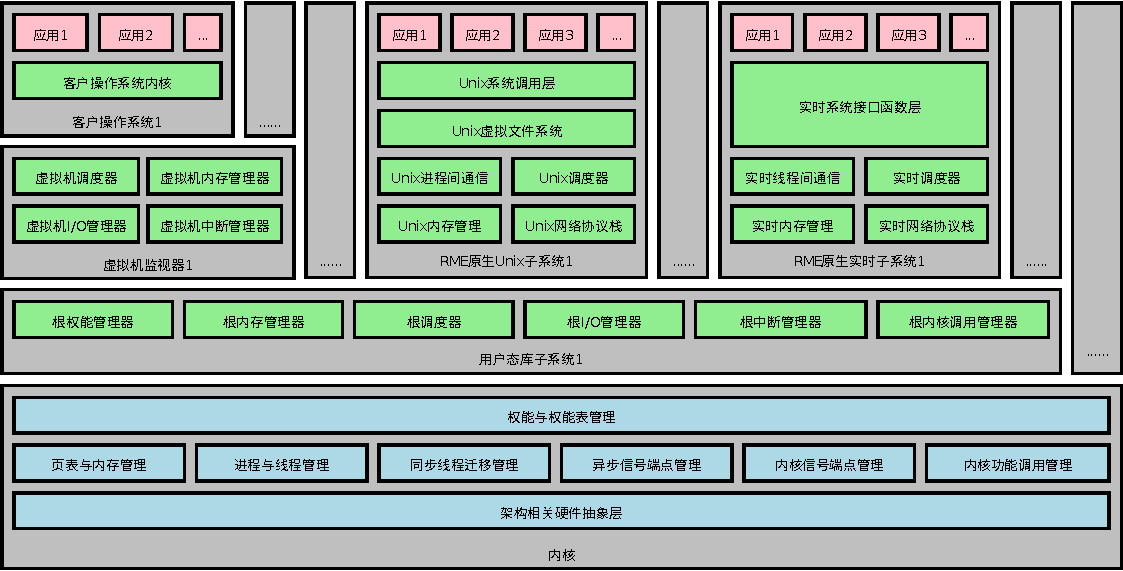
\includegraphics[width=0.90\textwidth]{Figure/image4.pdf}
    \caption{RME简略架构总览}
    \label{fig:1-3-rme-architecture-overview}
\end{figure}

\section{本章参考文献}\label{sec:1-bibliography}

\protect\phantomsection\label{cite:1-1}

\noindent {[}1{]} T. N. B. Anh and S.-L. Tan, ``Real-time operating systems for small microcontrollers,'' \textit{IEEE Micro}, vol. 29, 2009.

\protect\phantomsection\label{cite:1-2}

\noindent {[}2{]} R. P. Kar, ``Implementing the Rhealstone real-time benchmark,'' \textit{Dr. Dobb's Journal}, vol. 15, pp. 46--55, 1990.

\protect\phantomsection\label{cite:1-3}

\noindent {[}3{]} T. J. Boger, ``Rhealstone benchmarking of FreeRTOS and the Xilinx Zynq extensible processing platform,'' M.S. thesis, Temple University, 2013.

\protect\phantomsection\label{cite:1-4}

\noindent {[}4{]} G. Klein, K. Elphinstone, G. Heiser, J. Andronick, D. Cock, P. Derrin, et al., ``seL4: formal verification of an OS kernel,'' in \textit{Proceedings of the ACM SIGOPS 22nd Symposium on Operating Systems Principles}, Big Sky, MT, USA, 2009.

\protect\phantomsection\label{cite:1-5}

\noindent {[}5{]} U. Steinberg and B. Kauer, ``NOVA: a microhypervisor-based secure virtualization architecture,'' in \textit{Proceedings of the 5th European Conference on Computer Systems}, 2010, pp. 209--222.

